\section{Presentation of poperties of quantum walks}

In this chapter, I review classical and quantum walking on three specific graphs, for which interesting results can be observed. I discuss the evolution of the probability distributions and the hitting and mixing times for classical and quantum walks with the Hadamard, Grover and Fourier (DFT) coins.

\subsection{Walks on the line}

The first graph to be reviewed is the line (with $100$ vertices), using the adjacency matrix below. It is important to note, that an extra edge has to be added to connect the two ends of the line (see Theorem (\ref{PermutationMatricesTheorem}) for details).

\begin{figure}[H]
\centering
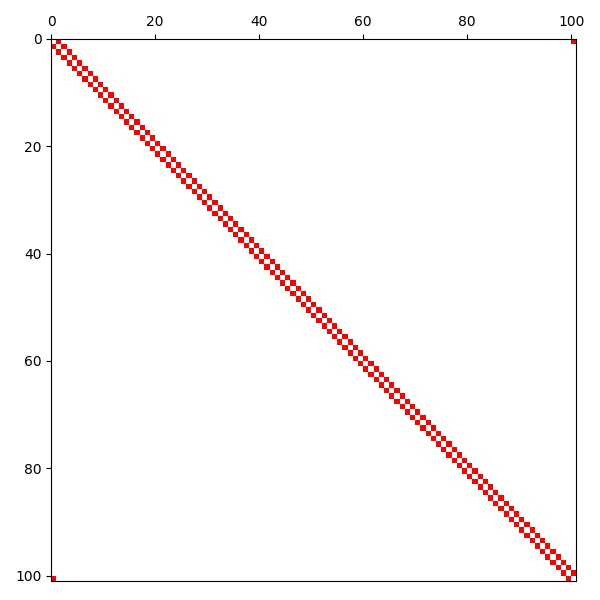
\includegraphics[width=0.5\linewidth]{./figures/results/path/graph.jpg}
\caption{Adjacency matrix of the line}
\end{figure}

In the following pictures, we can see the changes in the probability distribution during the walk. The $x$ axis contains the vertices, and the $y$ axis contains the steps. The walker starts from the centre, and in the classical case, multiple runs are done to arrive at a probability distribution, while in the quantum case, a single walker is enough, as it spreads in superposition over the graph.

The ballistic nature of the walk can be seen from steps $0$ to $50$, where the bright yellow diagonals represent a strong probability concentration spreading to the two ends of the line. When the probability bumps reach the sides, they cross over and travel to the opposite ends.

From steps $50$ to $200$, we can see secondary, tertiary, and further yellow bumps travelling alongside the main ones. These reach the ends slower and cross over each other later. This results in a beautiful weaved pattern in the picture.

Since the line is a $2$-regular graph, $2$ dimensional coins are used. The 2 dimensional Hadamard-coin and Fourier-coin are identical, while the 2 dimensional Grover-coin results in the walker not moving away from the
starting position, hence why only the Hadmard coin is shown in the distributions.

\begin{figure}[H]
  \centering
  \begin{subfigure}{.45\linewidth}
    \centering
    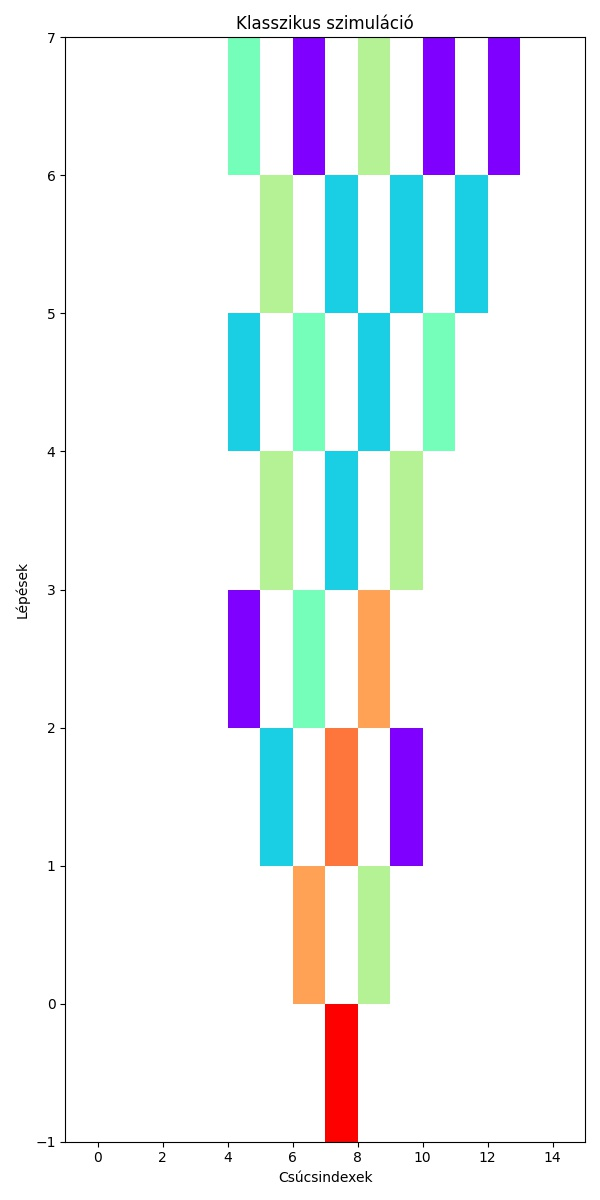
\includegraphics[width=\linewidth]{./figures/results/path/classical.jpg}
    \caption{Classical walk}
  \end{subfigure}
  \begin{subfigure}{.45\linewidth}
    \centering
    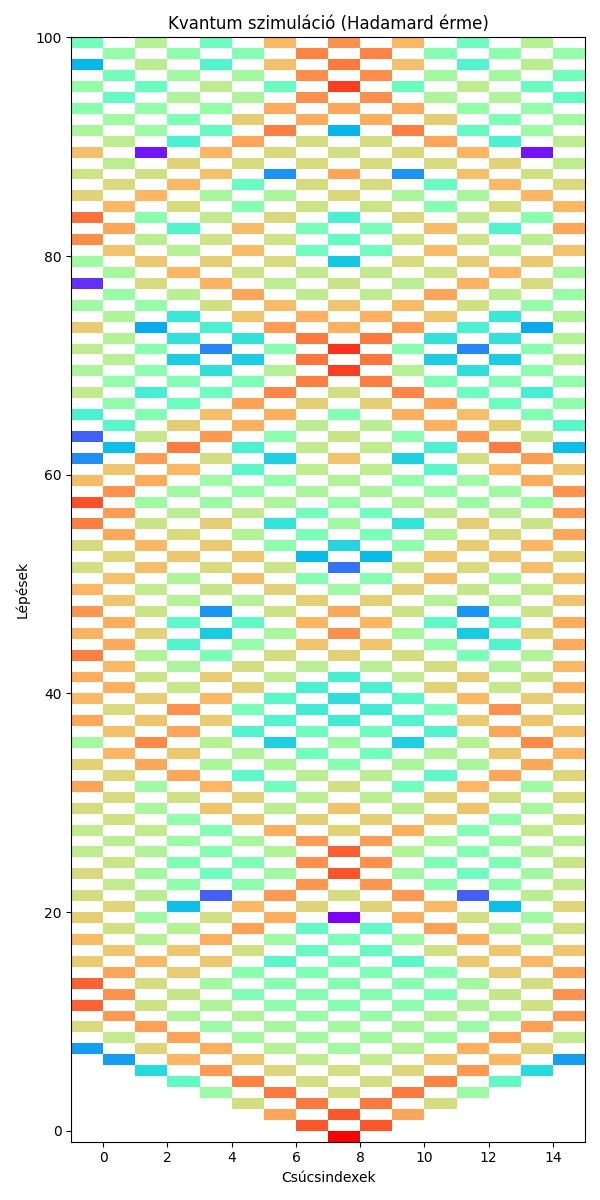
\includegraphics[width=\linewidth]{./figures/results/path/hadamard.jpg}
    \caption{Quantum walk with the Hadamard coin}
  \end{subfigure}
  \caption{Probability distribution of classical and quantum walks on the line}
\end{figure}

I have empirically measured hitting and mixing times for the different types of walks. Hitting time
is the expected number of steps to reach a specific vertex from the starting point. For this, I have
plotted the number of steps it took to first reach a particular vertex from the starting point. Mixing
time is the number of steps it takes before reaching the stationary distribution with $\varepsilon$ error.
For this, I have plotted the Euclidean difference between the walk's current and the end distribution.

In the following pictures, we can see the classical hitting and mixing times. Since my classical simulator approximates the distribution by running multiple walkers, the hitting time is slightly asymmetric. We can see from comparing the classical and the quantum hitting times that the quantum walk spreads faster than the classical one.

On the classical mixing time, we can see that the walker has not reached the stationary distribution. This is because until the walker reaches the ends of the line, the graph is essentially bipartite with two different limiting distributions and only after crossing over to the other side can the walk spread uniformly. This can also be seen in the probability distribution image above. At around step $300$, the colour of the image intensifies at the sides. Before that, the distribution alternates between odd and even indexes having $0$ probability, resulting in a chessboard pattern of white and colorful rectangles.

The quantum walk is mixing much better, as can be seen by the mixing time and the distribution image as well.

\begin{figure}[H]
  \centering
  \begin{subfigure}{.45\linewidth}
    \centering
    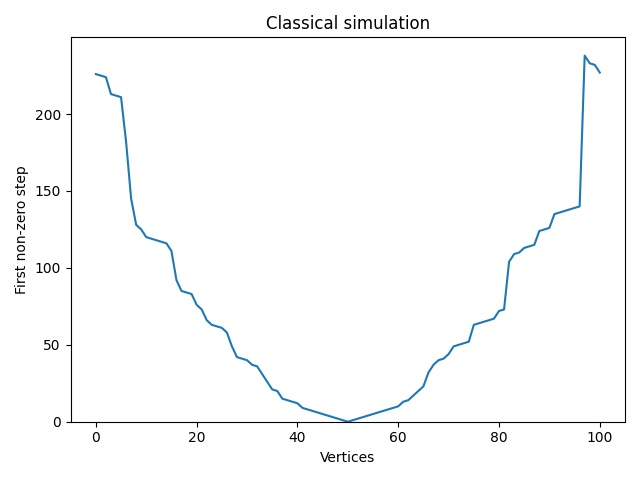
\includegraphics[width=\linewidth]{./figures/results/path/classical_hitting_time.jpg}
    \caption{Classical hitting time}
  \end{subfigure}
  \begin{subfigure}{.45\linewidth}
    \centering
    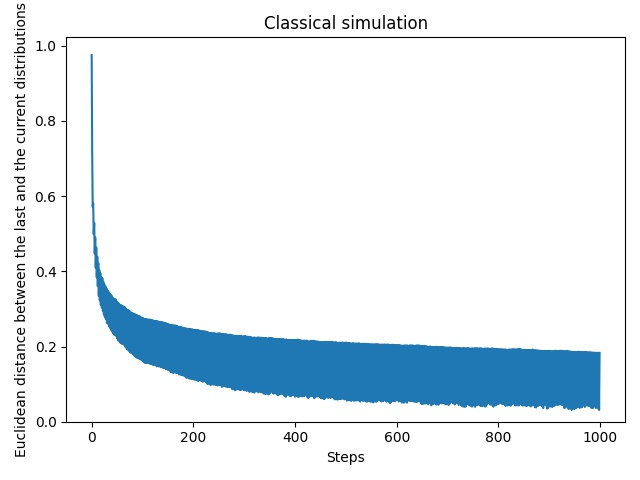
\includegraphics[width=\linewidth]{./figures/results/path/classical_mixing_time.jpg}
    \caption{Classical mixing time}
  \end{subfigure}
  \caption{Classical hitting and mixing times on the line}
\end{figure}

\begin{figure}[H]
  \centering
  \begin{subfigure}{.45\linewidth}
    \centering
    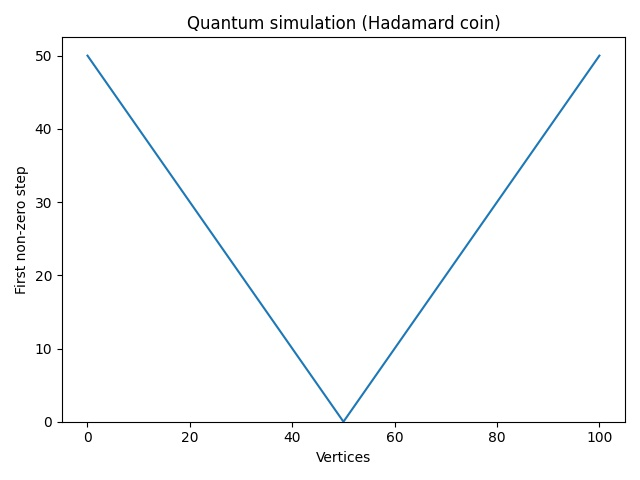
\includegraphics[width=\linewidth]{./figures/results/path/hadamard_hitting_time.jpg}
    \caption{Hadamard hitting time}
  \end{subfigure}
  \begin{subfigure}{.45\linewidth}
    \centering
    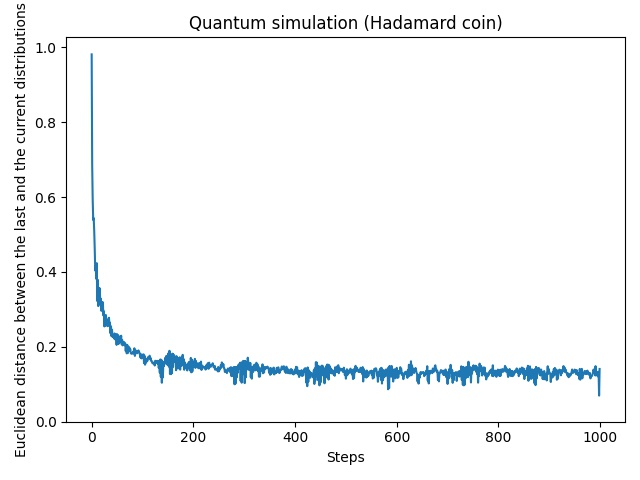
\includegraphics[width=\linewidth]{./figures/results/path/hadamard_mixing_time.jpg}
    \caption{Hadamard mixing time}
  \end{subfigure}
  \caption{Quantum (Hadamard) hitting and mixing times on the line}
\end{figure}

\subsection{Walks on the grid}

The second graph reviewed is the 2 dimensional grid (with $4\times{}4=16$ vertices), using the adjacency matrix below.

\begin{figure}[H]
\centering
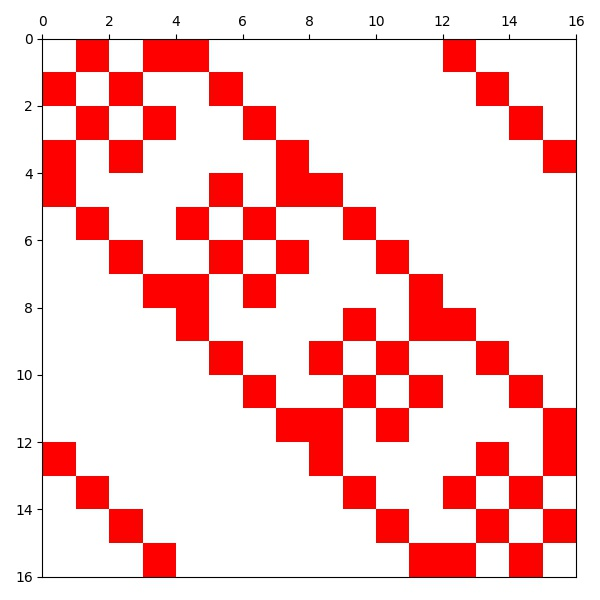
\includegraphics[width=0.5\linewidth]{./figures/results/grid/graph.jpg}
\caption{Adjacency matrix of the grid}
\end{figure}

The following 4 images contain the classical, the quantum Hadamard, the quantum Grover and the quantum Fourier walks on the grid. The classical walk quickly spreads over the graph since all vertices are close to each other (as opposed to the line, where the maximum distance is large).

In the quantum case, using the Hadamard and Grover coins, an important quality of the quantum walks can be distinctly observed: quantum walks are periodic since the eigenvalues of the evolution operator are complex roots of unity. Furthermore, by choosing a vertex count that is a power of $2$, I was able to create an evolution operator that has specific eigenvalues that result in the walker returning to its starting position
with $100\%$ probability (see the repeated red rectangles in the images), showing the cyclic nature of the quantum walk.

The Fourier coin mixes the state much better, resulting in no specific order in that image.

\begin{figure}[H]
  \centering
  \begin{subfigure}{.45\linewidth}
    \centering
    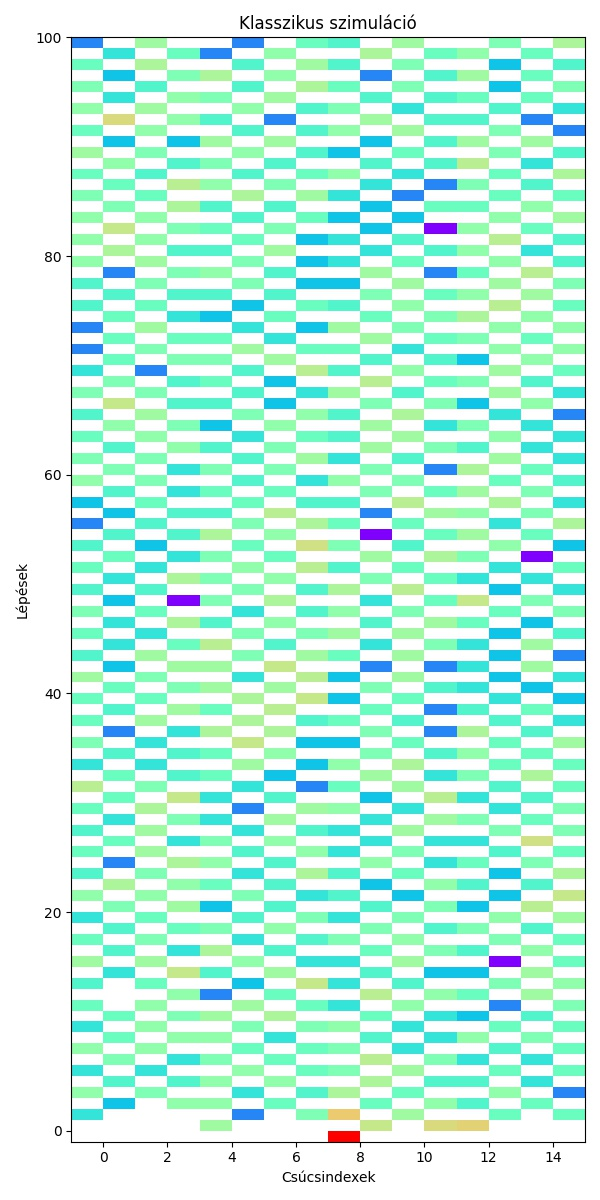
\includegraphics[width=\linewidth]{./figures/results/grid/classical.jpg}
    \caption{Classical walk}
  \end{subfigure}
  \begin{subfigure}{.45\linewidth}
    \centering
    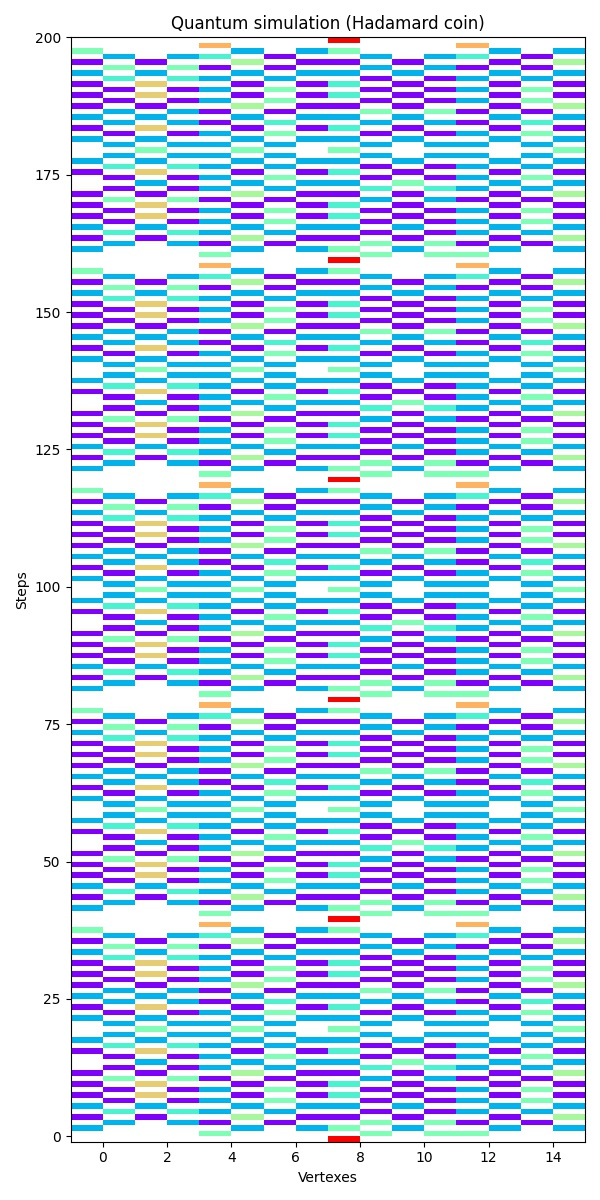
\includegraphics[width=\linewidth]{./figures/results/grid/hadamard.jpg}
    \caption{Quantum walk with the Hadamard coin}
  \end{subfigure}
  \caption{Probability distribution of classical and quantum walks on the grid}
\end{figure}

\begin{figure}[H]
  \centering
  \begin{subfigure}{.45\linewidth}
    \centering
    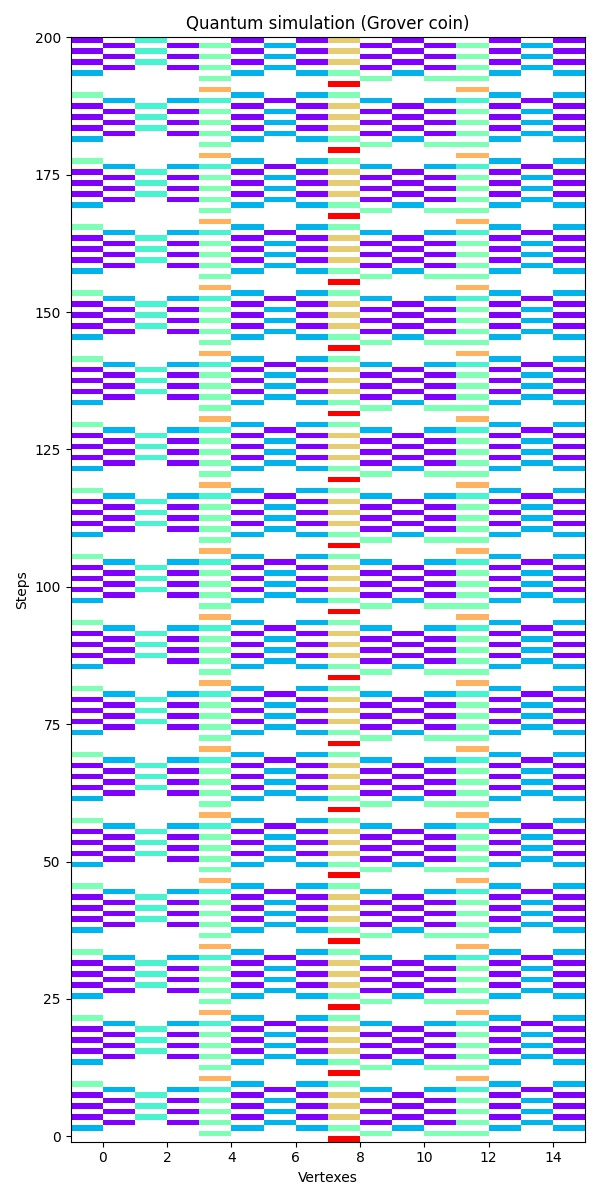
\includegraphics[width=\linewidth]{./figures/results/grid/grover.jpg}
    \caption{Quantum walk with the Grover coin}
  \end{subfigure}
  \begin{subfigure}{.45\linewidth}
    \centering
    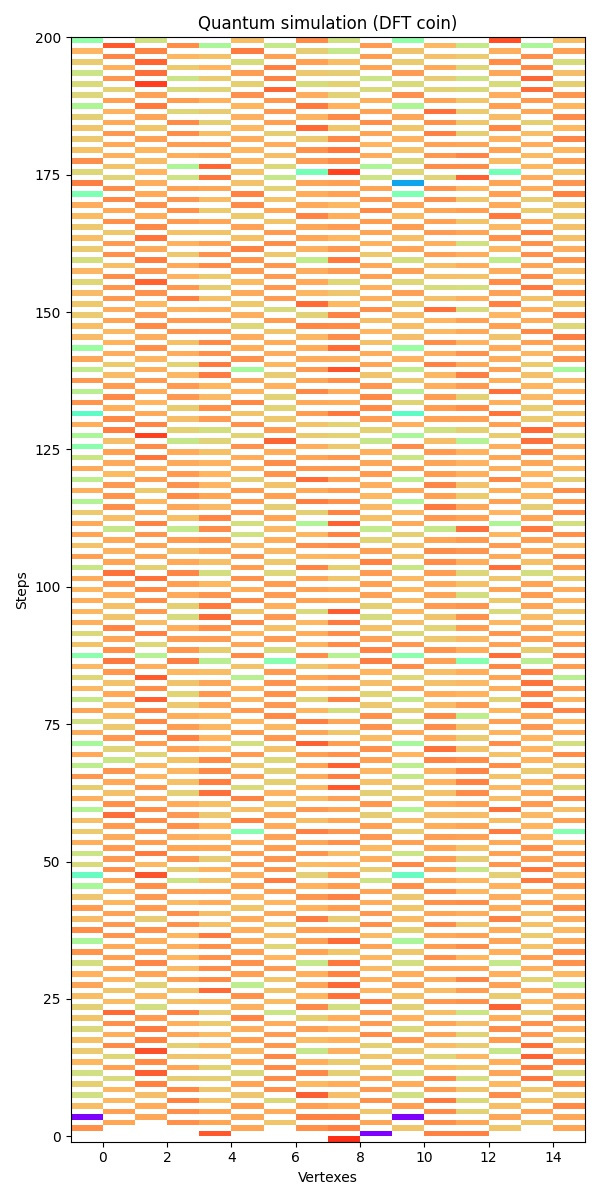
\includegraphics[width=\linewidth]{./figures/results/grid/dft.jpg}
    \caption{Quantum walk with the Fourier coin}
  \end{subfigure}
  \caption{Probability distribution of quantum walks on the grid}
\end{figure}

Interestingly, the hitting times of the 4 walks are similar. This is probably due to the fact, that the
graph is small, which allows the classical walk to spread just as quickly as its quantum counterpart. We can see, that neither of the walks reached a stationary distribution. In the quantum case, we know that the walks
are periodic, so there is no stationary distribution, while in the classical case, the graph is bipartite.

\begin{figure}[H]
  \centering
  \begin{subfigure}{.45\linewidth}
    \centering
    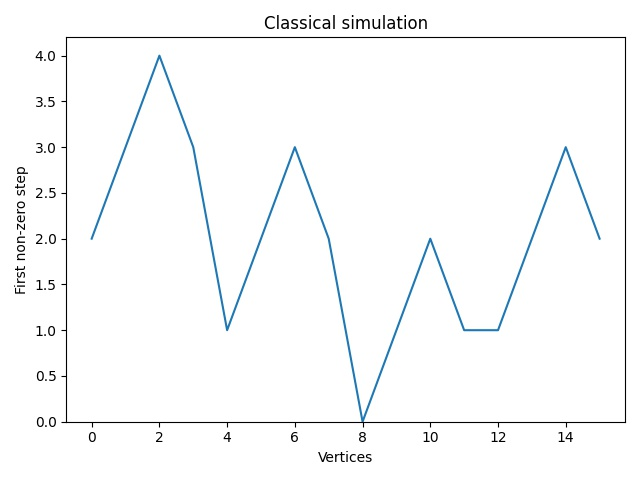
\includegraphics[width=\linewidth]{./figures/results/grid/classical_hitting_time.jpg}
    \caption{Classical hitting time}
  \end{subfigure}
  \begin{subfigure}{.45\linewidth}
    \centering
    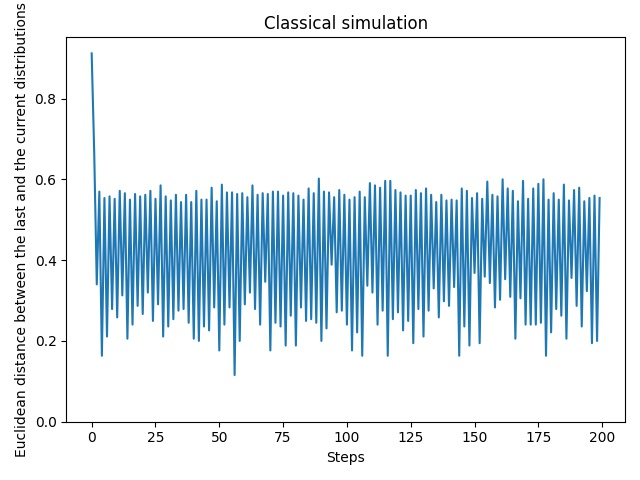
\includegraphics[width=\linewidth]{./figures/results/grid/classical_mixing_time.jpg}
    \caption{Classical mixing time}
  \end{subfigure}
  \caption{Classical hitting and mixing times on the grid}
\end{figure}

\begin{figure}[H]
  \centering
  \begin{subfigure}{.45\linewidth}
    \centering
    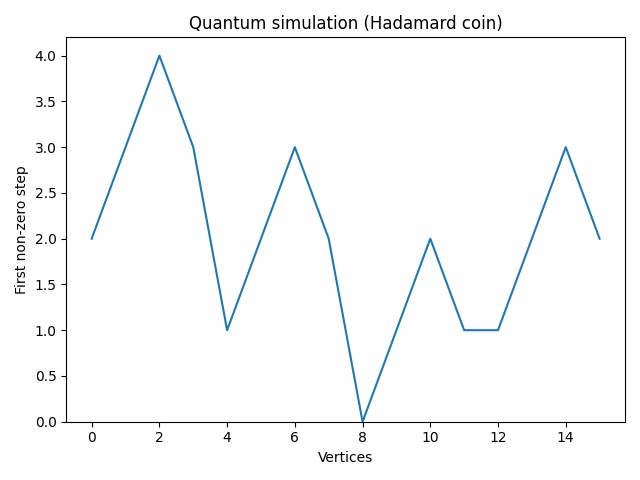
\includegraphics[width=\linewidth]{./figures/results/grid/hadamard_hitting_time.jpg}
    \caption{Hadamard hitting time}
  \end{subfigure}
  \begin{subfigure}{.45\linewidth}
    \centering
    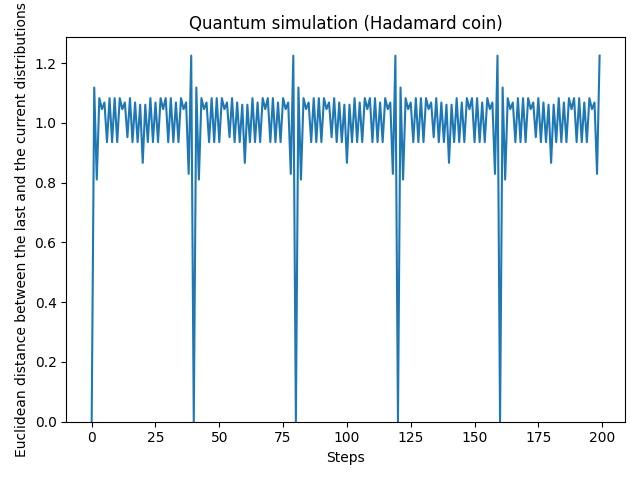
\includegraphics[width=\linewidth]{./figures/results/grid/hadamard_mixing_time.jpg}
    \caption{Hadamard mixing time}
  \end{subfigure}
  \caption{Quantum (Hadamard) hitting and mixing times on the grid}
\end{figure}

\begin{figure}[H]
  \centering
  \begin{subfigure}{.45\linewidth}
    \centering
    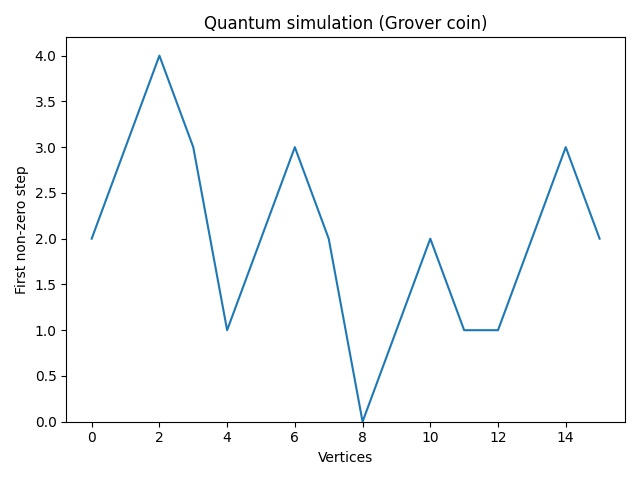
\includegraphics[width=\linewidth]{./figures/results/grid/grover_hitting_time.jpg}
    \caption{Grover hitting time}
  \end{subfigure}
  \begin{subfigure}{.45\linewidth}
    \centering
    \includegraphics[width=\linewidth]{./figures/results/grid/grover_mixing_time.jpg}
    \caption{Grover mixing time}
  \end{subfigure}
  \caption{Quantum (Grover) hitting and mixing times on the grid}
\end{figure}

\begin{figure}[H]
  \centering
  \begin{subfigure}{.45\linewidth}
    \centering
    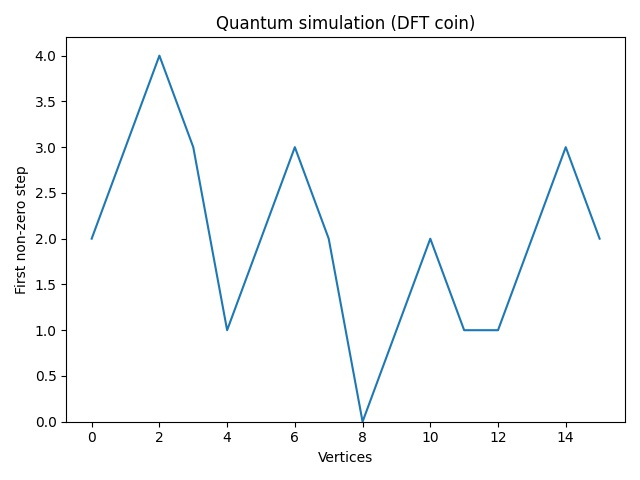
\includegraphics[width=\linewidth]{./figures/results/grid/dft_hitting_time.jpg}
    \caption{Fourier hitting time}
  \end{subfigure}
  \begin{subfigure}{.45\linewidth}
    \centering
    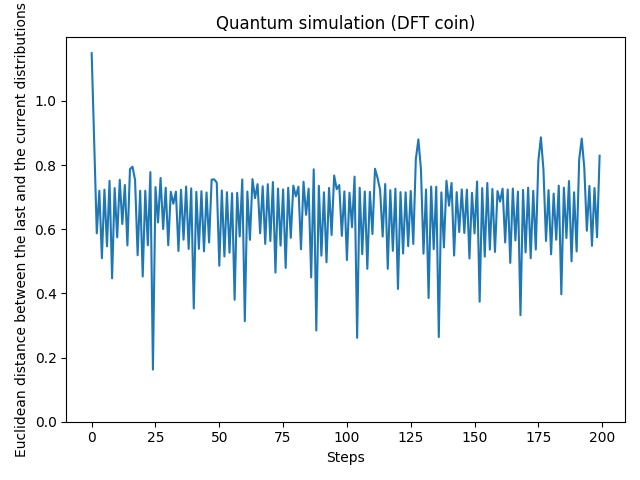
\includegraphics[width=\linewidth]{./figures/results/grid/dft_mixing_time.jpg}
    \caption{Fourier mixing time}
  \end{subfigure}
  \caption{Quantum (Fourier) hitting and mixing times on the grid}
\end{figure}

\subsection{Walks on hypercube}

The third graph reviewed is the 4 dimensional boolean hypercube (with $2^4 = 16$ vertices), using the adjacency matrix below.

\begin{figure}[H]
\centering
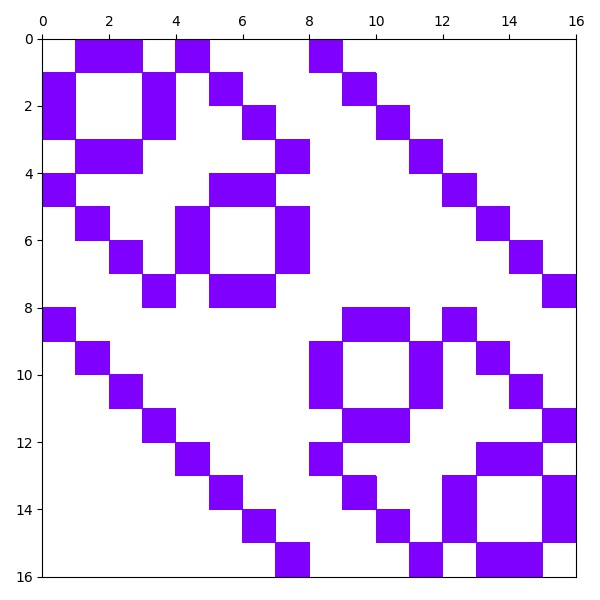
\includegraphics[width=0.5\linewidth]{./figures/results/hypercube/graph.jpg}
\caption{Adjacency graph of the hypercube}
\end{figure}

Similarly to the grid, the walks are recurrent (cyclic) in the Hadamard and Grover case. Interestingly in this case the periodicity can be visibly observed with the Fourier coin, however the walk does not return to its
original starting point with $100\%$ probability. This is due to the eigenvalues of the evolution operator
just being slightly off, so there is no small exponent for which the evolution operator is the identity.

\begin{figure}[H]
  \centering
  \begin{subfigure}{.45\linewidth}
    \centering
    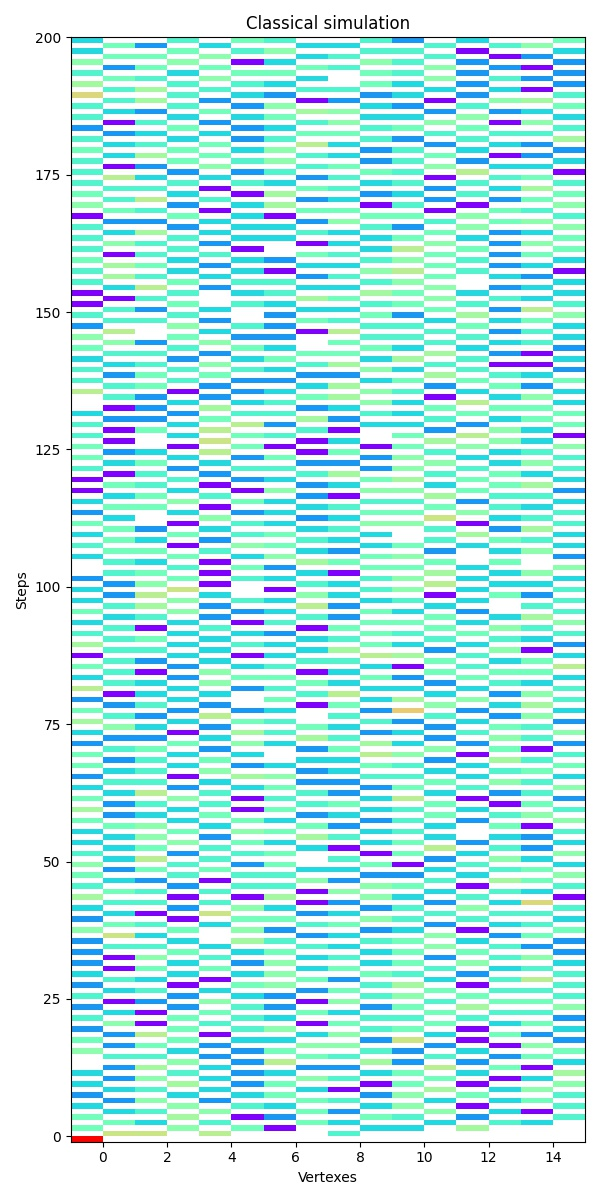
\includegraphics[width=\linewidth]{./figures/results/hypercube/classical.jpg}
    \caption{Classical walk}
  \end{subfigure}
  \begin{subfigure}{.45\linewidth}
    \centering
    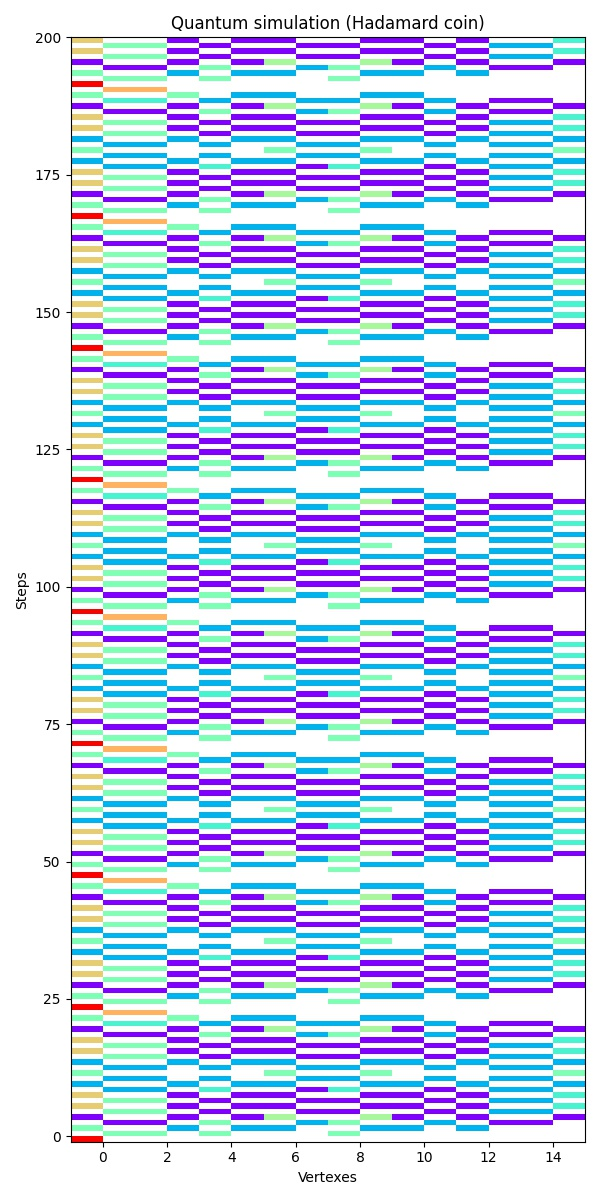
\includegraphics[width=\linewidth]{./figures/results/hypercube/hadamard.jpg}
    \caption{Quantum walk with the Hadamard coin}
  \end{subfigure}
  \caption{Probability distribution of classical and quantum walks on the hypercube}
\end{figure}

\begin{figure}[H]
  \centering
  \begin{subfigure}{.45\linewidth}
    \centering
    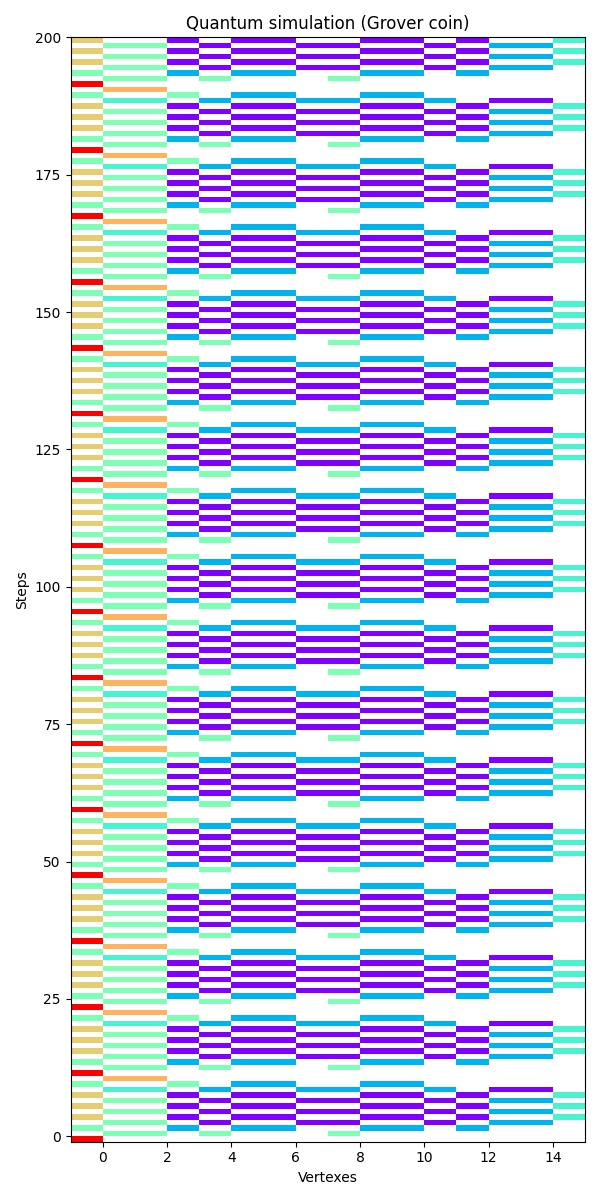
\includegraphics[width=\linewidth]{./figures/results/hypercube/grover.jpg}
    \caption{Quantum walk with the Grover coin}
  \end{subfigure}
  \begin{subfigure}{.45\linewidth}
    \centering
    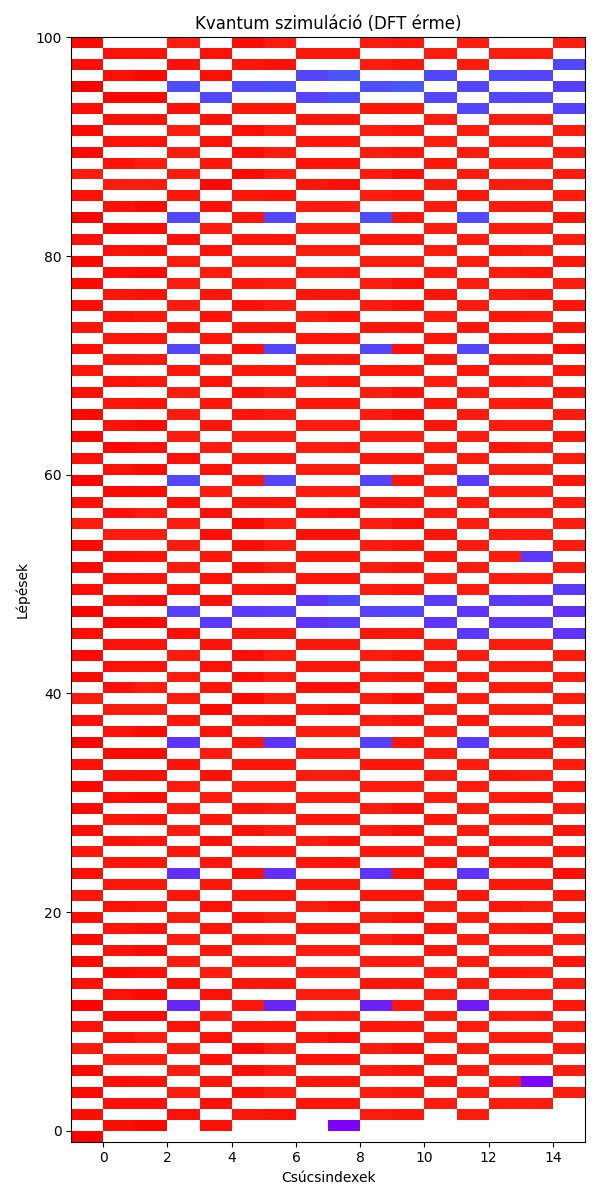
\includegraphics[width=\linewidth]{./figures/results/hypercube/dft.jpg}
    \caption{Quantum walk with the Fourier coin}
  \end{subfigure}
  \caption{Probability distribution of quantum walks on the hypercube}
\end{figure}

Similarly to the grid, the hitting times are identical, since the graph is small and the classical walk's
disadvantage is not visible. The hypercube is also bipartite, resulting in no stationary distribution for the
classical walk either.

\begin{figure}[H]
  \centering
  \begin{subfigure}{.45\linewidth}
    \centering
    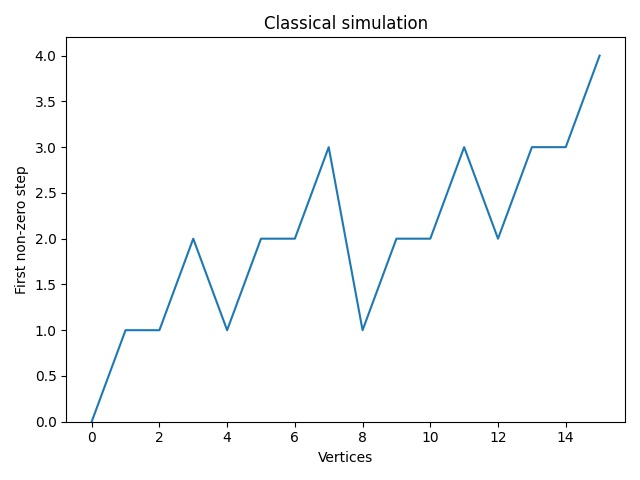
\includegraphics[width=\linewidth]{./figures/results/hypercube/classical_hitting_time.jpg}
    \caption{Classical hitting time}
  \end{subfigure}
  \begin{subfigure}{.45\linewidth}
    \centering
    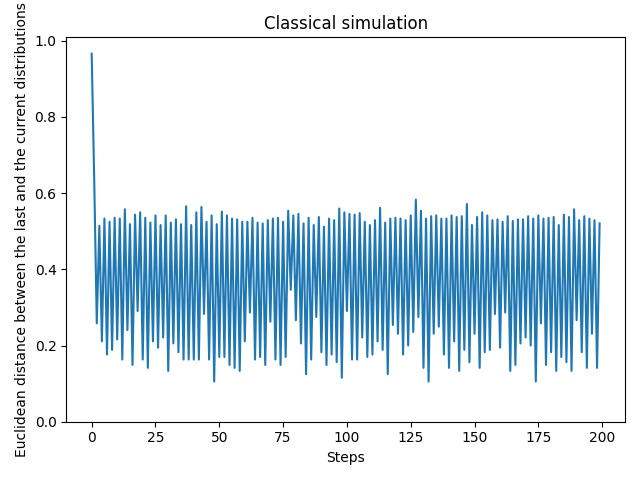
\includegraphics[width=\linewidth]{./figures/results/hypercube/classical_mixing_time.jpg}
    \caption{Classical mixing time}
  \end{subfigure}
  \caption{Classical hitting and mixing times on the hypercube}
\end{figure}

\begin{figure}[H]
  \centering
  \begin{subfigure}{.45\linewidth}
    \centering
    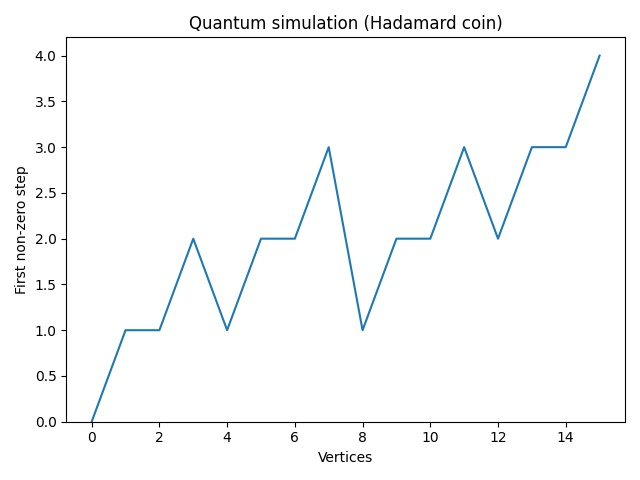
\includegraphics[width=\linewidth]{./figures/results/hypercube/hadamard_hitting_time.jpg}
    \caption{Hadamard hitting time}
  \end{subfigure}
  \begin{subfigure}{.45\linewidth}
    \centering
    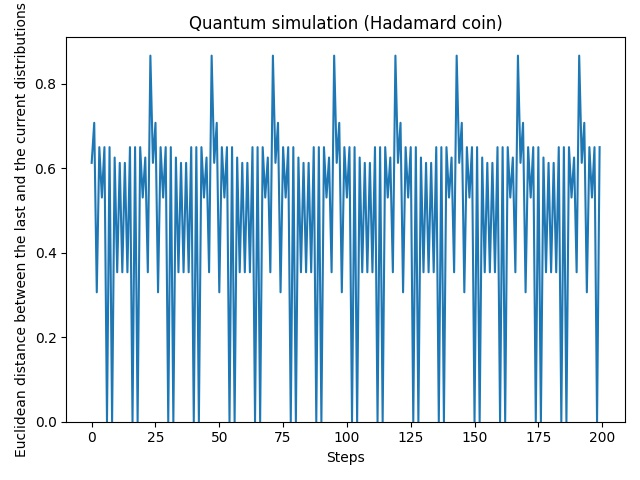
\includegraphics[width=\linewidth]{./figures/results/hypercube/hadamard_mixing_time.jpg}
    \caption{Hadamard mixing time}
  \end{subfigure}
  \caption{Quantum (Hadamard) hitting and mixing times on the hypercube}
\end{figure}

\begin{figure}[H]
  \centering
  \begin{subfigure}{.45\linewidth}
    \centering
    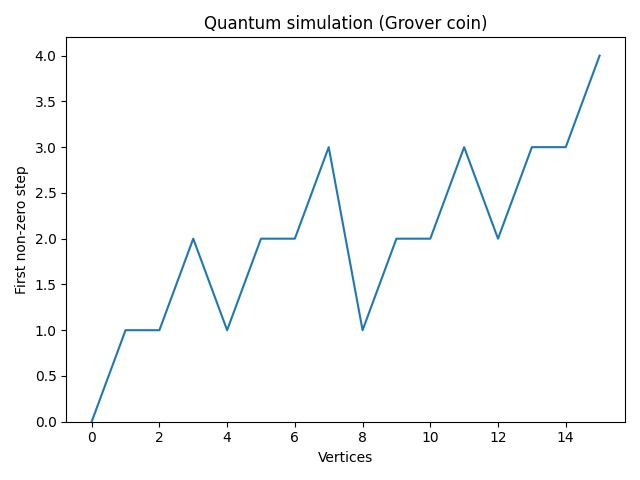
\includegraphics[width=\linewidth]{./figures/results/hypercube/grover_hitting_time.jpg}
    \caption{Grover hitting time}
  \end{subfigure}
  \begin{subfigure}{.45\linewidth}
    \centering
    \includegraphics[width=\linewidth]{./figures/results/hypercube/grover_mixing_time.jpg}
    \caption{Grover mixing time}
  \end{subfigure}
  \caption{Quantum (Grover) hitting and mixing times on the hypercube}
\end{figure}

\begin{figure}[H]
  \centering
  \begin{subfigure}{.45\linewidth}
    \centering
    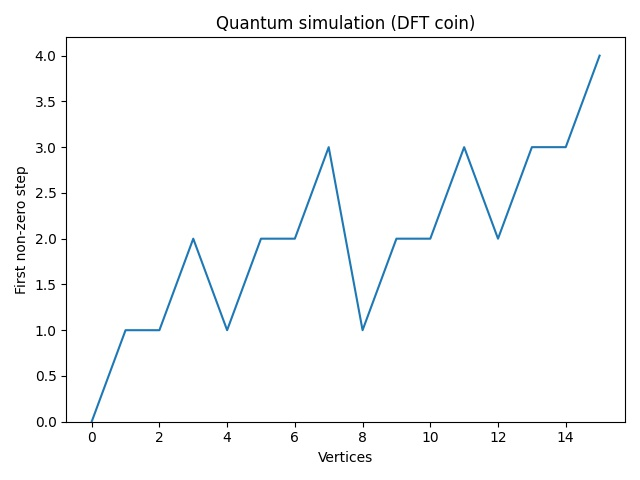
\includegraphics[width=\linewidth]{./figures/results/hypercube/dft_hitting_time.jpg}
    \caption{Fourier hitting time}
  \end{subfigure}
  \begin{subfigure}{.45\linewidth}
    \centering
    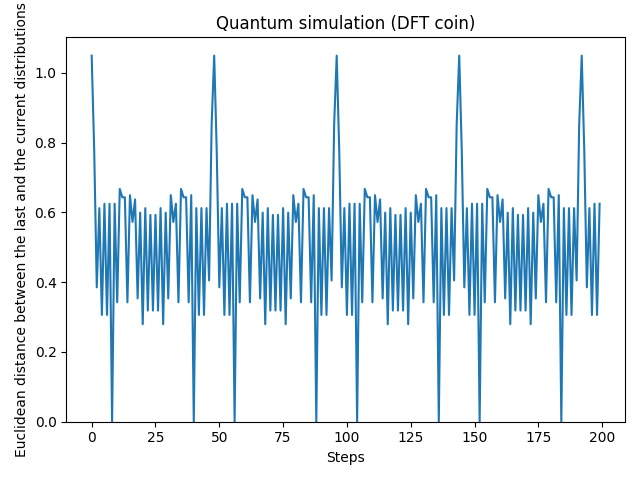
\includegraphics[width=\linewidth]{./figures/results/hypercube/dft_mixing_time.jpg}
    \caption{Fourier mixing time}
  \end{subfigure}
  \caption{Quantum (Fourier) hitting and mixing times on the hypercube}
\end{figure}
